%% CELERIS -- long-form methods & validation report (arXiv preprint; physics.comp-ph).
%% The journal paper is the short JOSS paper in ../paper.md; this is its companion
%% technical report (formerly drafted for CPC), NOT a second journal submission.
%% Document class: Elsevier elsarticle. Bibliography: elsarticle-num (../paper.bib).
%% Build (from paper/longform/):
%%   pdflatex paper  ->  bibtex paper  ->  pdflatex paper  ->  pdflatex paper
\documentclass[preprint,12pt]{elsarticle}

\usepackage[T1]{fontenc}
\usepackage{amsmath}
\usepackage{amssymb}
\usepackage{graphicx}
\usepackage{booktabs}
\usepackage{pifont}
\usepackage{url}
\usepackage{tikz}
\usetikzlibrary{positioning,arrows.meta}

% Double square brackets for the Toeplitz convolution matrices (no extra package).
\providecommand{\llbracket}{[\![}
\providecommand{\rrbracket}{]\!]}

% Feature-table glyphs.
\newcommand{\yes}{\ding{51}}          % provided
\newcommand{\no}{\ding{55}}           % not provided
\newcommand{\pt}{$\sim$}              % partial / possible with user code
\newcommand{\na}{---}                 % not applicable

\journal{arXiv (physics.comp-ph)}
\graphicspath{{../}}

\begin{document}

\begin{frontmatter}

\title{CELERIS: an integrated, validated RCWA pipeline for metalens
design, analysis, and fabrication layout}

\author[ucf]{Amarnath Patel\corref{cor1}}
\ead{am397421@ucf.edu}
\cortext[cor1]{Corresponding author.}
\affiliation[ucf]{organization={University of Central Florida},
                  city={Orlando}, state={FL}, country={USA}}

\begin{abstract}
Metasurfaces and metalenses --- flat optical elements built from subwavelength
scatterers (``meta-atoms'') --- are designed by (i) solving Maxwell's equations
for a periodic unit cell to build a library of meta-atom responses, (ii) mapping
a target optical phase profile onto that library, (iii) analyzing the resulting
device's optical performance, and (iv) exporting a mask layout for fabrication.
The standard rigorous electromagnetic method for step (i) is rigorous coupled-wave
analysis (RCWA), also known as the Fourier modal method (FMM). \textbf{CELERIS} is
a from-scratch, validated implementation of this full workflow in a single
native package. It couples a C++23 RCWA engine (1D and 2D-vectorial, with Li/Liu--Fan
Fourier factorization and a Redheffer S-matrix stack) to a meta-atom library builder,
a phase-mapping and inverse-design layer (including achromatic and Pancharatnam--Berry
designs), a full optical analysis battery (Strehl ratio, PSF, MTF, wavefront/Zernike,
through-focus, chromatic, field-resolved, and tolerance analyses), GPU-accelerated
far-field propagation, and fabrication-ready GDSII export. It is scriptable from C++,
a command-line interface, and Python (via pybind11), and ships with a desktop GUI.
Correctness is enforced by a locked self-test suite (20+ cases) cross-checked against
closed-form physics (Fresnel/TMM, effective-medium theory), energy conservation, and
independent RCWA solvers (\texttt{grcwa} and Stanford~S$^4$). The pipeline is
demonstrated by reproducing a canonical published TiO$_2$ metalens end to end and by
computing the \emph{group-delay design limit} that bounds single-etch broadband
achromats---an aperture--bandwidth ceiling that emerges only from the coupled library,
design, and analysis stages, not from any solver kernel alone---and recovering it for a
published broadband achromat. A sweep of 36 single-etch libraries (three materials, two
phase mechanisms, six heights) then maps how much of the Presutti--Monticone
delay--bandwidth bound such libraries reach (13--68\%, levelling off at about 30--55\%
for etch depths of $0.8~\mu$m and more), and shows that span-based
aperture estimates overstate propagation-phase achromats by about a factor of two.
\end{abstract}

\begin{keyword}
metasurface \sep metalens \sep rigorous coupled-wave analysis \sep
Fourier modal method \sep inverse design \sep GDSII
\end{keyword}

\end{frontmatter}

%% ---------------------------------------------------------------------------
\section*{Program summary}
\begin{description}
\item[Program title:] CELERIS
\item[Developer's repository link:] \url{https://github.com/jeebuscrossaint/CELERIS}
\item[Licensing provisions:] Apache License 2.0
\item[Permanent archive:] Zenodo (v1.0.0): \url{https://doi.org/10.5281/zenodo.21891346};
      concept DOI (always latest version): \url{https://doi.org/10.5281/zenodo.21891345}
\item[Programming languages:] C++23 (engine), CUDA (optional GPU far-field kernel),
      Python (pybind11 bindings)
\item[No.\ of lines in distributed program:] $\approx$14{,}000 (C++23/CUDA/Python;
      excludes the bundled Dear ImGui and the configure-time-fetched Eigen).
\item[Distribution format:] Git repository and \texttt{.tar.gz} source archive
      (Apache-2.0), permanently archived on Zenodo (DOIs above).
\item[External routines/libraries:] Eigen (required, header-only, fetched at configure
      time); optional Intel MKL (CPU acceleration), CUDA (GPU far-field), pybind11
      (Python module), Dear ImGui (desktop GUI).
\item[Nature of problem:] Designing a metalens/metasurface requires solving Maxwell's
      equations for periodic subwavelength unit cells, assembling a meta-atom library,
      mapping a target optical phase profile onto it, analyzing the resulting device's
      optical performance, and exporting a fabrication mask --- a multi-stage workflow
      that existing RCWA solvers do not provide end to end.
\item[Solution method:] Rigorous coupled-wave analysis / Fourier modal method (1D and
      2D-vectorial) with Li/Liu--Fan Fourier factorization and a Redheffer S-matrix
      layer recursion, wrapped in a library builder, a phase-mapping / inverse-design
      layer (including achromatic and Pancharatnam--Berry recipes), an optical analysis
      battery, GPU-accelerated far-field propagation, and GDSII layout export.
\item[Dependencies:] Eigen (header-only, fetched at configure time); optional Intel MKL
      and CUDA for acceleration; pybind11 for the Python module. Validated against
      \texttt{grcwa} and Stanford~S$^4$.
\item[Restrictions:] Scope is metalenses/metasurfaces via RCWA (not FDTD or ray
      tracing). The modal eigensolve runs on the CPU; the GPU accelerates far-field
      propagation only.
\item[Operating systems:] Linux and Windows (CPU build has no external runtime
      dependencies). Requires a C++23 compiler with \texttt{<print>}/\texttt{std::format}
      support --- GCC~$\geq$~14 (as used in CI) or a comparably recent MSVC/Clang.
\item[Running time:] Seconds for a complete monochromatic metalens design: a
      $20\,\mu$m-aperture, $f=50\,\mu$m lens (a $57\times57$ meta-atom layout with
      full focal analysis and GDSII export) completes in $\approx$2.5\,s on a single
      CPU core. The locked validation suite ($\sim$25 checks, including the 2D
      convergence study) runs in $\approx$90\,s on 16 cores. Wall time is dominated
      by the per-unit-cell modal eigensolve and scales with the truncation order.
\end{description}

%% ---------------------------------------------------------------------------
\section{Introduction}
Metasurfaces --- planar arrays of subwavelength scatterers that impose an
engineered, spatially varying response on an incident wavefront --- have reshaped
optical component design over the past decade, replacing bulk refractive elements
with lithographically defined flat optics~\cite{yu2011,yu2014flat,kildishev2013}.
By locally controlling phase, amplitude, and polarization, a single patterned layer
realizes lenses, deflectors, holograms, and polarization
optics~\cite{arbabi2015}. The metalens --- a flat focusing element built from a
radial phase profile --- is the canonical example and the motivating application of
this work: dielectric metalenses now reach high numerical aperture and high
efficiency, so the open design problems are chromatic correction and manufacturable
layout rather than the basic focusing principle.

Two design strategies recur throughout this literature and are built into CELERIS.
The first is the \emph{geometric} (Pancharatnam--Berry) phase~\cite{berry1984,bomzon2002}:
rotating a birefringent meta-atom imprints a wavelength-independent phase equal to
twice its orientation angle, a robust, dispersionless handle on the base phase
profile. The second is \emph{dispersion engineering} for broadband achromatic
focusing~\cite{aieta2015,wang2018}, in which the meta-atom library must supply not
only the correct phase at the center wavelength but the correct \emph{group delay}
across a band --- a requirement bounded, as Sec.~\ref{sec:method} makes precise, by a
physical aperture--bandwidth limit that a single-etch surface can span. Both
strategies require a rigorous electromagnetic solver in the loop, because the
meta-atom response is a full solution of Maxwell's equations in a
subwavelength-structured unit cell, not a thin-element phase mask. What has been
missing is not the solver but the validated machinery that turns it into a
fabricated, analyzed device; the remainder of this paper describes that pipeline and
its validation.

%% ---------------------------------------------------------------------------
\section{Statement of need}
Existing open-source RCWA codes --- S$^4$~\cite{liu2012s4}, RETICOLO~\cite{reticolo},
\texttt{grcwa}~\cite{grcwa}, TORCWA~\cite{torcwa}, \texttt{fmmax}~\cite{fmmax},
\texttt{meent}~\cite{meent} --- are \emph{solver kernels}: they compute the
electromagnetic response of a given periodic structure. Turning a solver into a
\emph{fabricated, analyzed metalens} still requires the user to hand-assemble the
surrounding workflow: sweeping a meta-atom library, mapping a phase profile onto it,
propagating to a focal plane, computing imaging metrics, running fabrication-tolerance
studies, and emitting a GDSII layout. Each researcher re-implements this scaffolding,
and the glue code is rarely validated or shared.

CELERIS provides that pipeline (Fig.~\ref{fig:pipeline}) as a single validated tool.
The target audience is
metasurface and metalens researchers who need to go from an optical specification
(focal length, aperture, wavelength, material) to a fabrication-ready, performance-
characterized design without stitching together a solver, a plotting stack, and a
layout tool. The contribution is not a new solver kernel but the \textbf{integration}
--- solver $\to$ library $\to$ design $\to$ analysis $\to$ layout --- validated
end to end against published devices.

The payoff of that integration is a capability, not merely a convenience. Because the
library builder, the group-delay design mapping, and the focal-plane analysis share one
data model, CELERIS computes the \emph{group-delay design limit} of a metalens: the
aperture--bandwidth product beyond which a single-etch achromat cannot focus
diffraction-limited across a band (Sec.~\ref{sec:method}, Eq.~\eqref{eq:gdspan}). This is
a property of the pipeline as a whole, not of any one solve --- a solver called in an
optimization loop returns unit-cell scattering coefficients, but not whether a target
device lies inside or outside the physically achievable region. Recovering this limit for
a published broadband achromat (Sec.~\ref{sec:validation}) is the paper's central
demonstration that an integrated, validated workflow yields device-level physics that a
bare kernel wrapped in a hand-written loop does not.

\begin{figure*}[t]
\centering
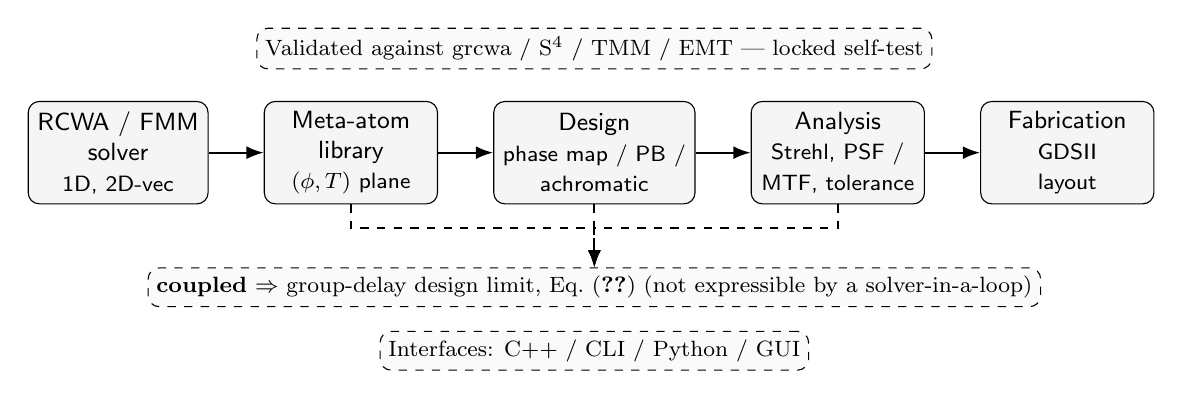
\begin{tikzpicture}[
  node distance=5mm and 7mm,
  stage/.style={draw, rounded corners, align=center, minimum height=13mm,
                minimum width=22mm, fill=black!4, font=\small\sffamily},
  io/.style={draw, dashed, rounded corners, align=center, font=\footnotesize,
             fill=black!2, inner sep=3pt},
  arr/.style={-{Latex[length=2.2mm]}, thick}]
  \node[stage] (solve)  {RCWA / FMM\\solver\\{\footnotesize 1D, 2D-vec}};
  \node[stage, right=of solve]  (lib)    {Meta-atom\\library\\{\footnotesize $(\phi,T)$ plane}};
  \node[stage, right=of lib]    (design) {Design\\{\footnotesize phase map / PB /}\\{\footnotesize achromatic}};
  \node[stage, right=of design] (ana)    {Analysis\\{\footnotesize Strehl, PSF /}\\{\footnotesize MTF, tolerance}};
  \node[stage, right=of ana]    (gds)    {Fabrication\\{\footnotesize GDSII}\\{\footnotesize layout}};
  \draw[arr] (solve)  -- (lib);
  \draw[arr] (lib)    -- (design);
  \draw[arr] (design) -- (ana);
  \draw[arr] (ana)    -- (gds);
  % one shared data model spanning all stages
  \node[io, below=8mm of design] (limit)
    {\textbf{coupled} $\Rightarrow$ group-delay design limit, Eq.~\eqref{eq:gdspan}
     (not expressible by a solver-in-a-loop)};
  \draw[arr, dashed] (lib.south)    -- ++(0,-3mm) -| (limit.north);
  \draw[arr, dashed] (design.south) -- (limit.north);
  \draw[arr, dashed] (ana.south)    -- ++(0,-3mm) -| (limit.north);
  % validation (top) + interfaces (bottom) bands, centered to avoid overlap
  \node[io, above=4mm of design] (val)
    {Validated against grcwa / S$^4$ / TMM / EMT --- locked self-test};
  \node[io, below=3mm of limit] (ifc)
    {Interfaces: C++ / CLI / Python / GUI};
\end{tikzpicture}
\caption{The CELERIS pipeline. The five stages share one data model, so the
integration is not glue but a capability: the coupling of the dispersive
$(\phi,T)$ library, the design map, and the focal analysis yields the group-delay
design limit (Sec.~\ref{sec:method}), a device-level result a bare solver called in
a loop cannot produce. The whole path is validated against independent solvers and
closed-form physics by a locked self-test.}
\label{fig:pipeline}
\end{figure*}

%% ---------------------------------------------------------------------------
\section{State of the field}
Table~\ref{tab:compare} positions CELERIS against widely used open RCWA/FMM
\emph{solver kernels}; the two integrated open metasurface pipelines closest to
CELERIS --- \texttt{metabox}~\cite{metabox} and \texttt{MetaCraft}~\cite{metacraft}
--- are discussed separately below, as they are design/optimization frameworks
rather than solver kernels. CELERIS deliberately \emph{does not} compete on automatic
differentiation (see Limitations); it competes on the forward analysis-and-design
battery that the solver kernels do not provide.

\begin{table*}[t]
\centering
\caption{Feature comparison (\yes~= provided, \pt~= partial/possible with user code,
\no~= not provided). Verified against each tool's documentation/publication; released
versions evolve, so cells should be re-checked at submission.}
\label{tab:compare}
\footnotesize
\setlength{\tabcolsep}{4pt}
\resizebox{\textwidth}{!}{%
\begin{tabular}{lccccccc}
\toprule
Feature & S$^4$ & RETICOLO & grcwa & TORCWA & fmmax & meent & \textbf{CELERIS} \\
\midrule
Language                        & C++/Lua/Py & MATLAB & Python & PyTorch & JAX & np/JAX/torch & \textbf{C++/Py} \\
License                         & GPL & (MATLAB) & GPL & LGPL & MIT & MIT & \textbf{Apache-2.0} \\
1D + 2D-vectorial RCWA          & \yes & \yes & \yes & \yes & \yes & \yes & \textbf{\yes} \\
Native GPU (full solve)         & \no & \no & \no & \yes & \yes & \yes & \textbf{\no~(far-field only)} \\
Automatic differentiation       & \no & \no & \yes & \yes & \yes & \yes & \textbf{\no~(FD; adjoint planned)} \\
Arbitrary meta-atom shapes      & \yes & \yes & \yes & \yes & \yes & \yes & \textbf{\yes} \\
Established user base / maturity & \yes & \yes & \pt & \pt & \pt & \pt & \textbf{\no~(new; v1.0)} \\
Integrated metalens \emph{design} & \pt & \pt & \pt & \pt & \pt & \pt & \textbf{\yes} \\
Optical \emph{analysis battery} & \no & \pt & \no & \no & \no & \no & \textbf{\yes} \\
Achromatic + PB design          & \no & \no & \no & \no & \no & \no & \textbf{\yes} \\
Fabrication-ready GDSII export  & \no & \no & \no & \no & \no & \no & \textbf{\yes} \\
Published-device reproductions  & \no & \no & \no & \no & \no & \no & \textbf{\yes} \\
Desktop GUI                     & \no & \no & \no & \no & \no & \no & \textbf{\yes} \\
\bottomrule
\end{tabular}%
}
\end{table*}

We state the trade-off plainly: the GPU/autodiff-native solvers (TORCWA, fmmax, meent)
are \emph{stronger solver kernels} --- they run the full modal solve on the GPU with
automatic differentiation, whereas CELERIS GPU-accelerates only far-field propagation
and optimizes by finite differences (an analytic adjoint is planned). CELERIS's contribution is orthogonal, and we state its boundary honestly. Open
pipelines that map a target phase onto an RCWA-characterized library and export GDSII
already exist: \texttt{metabox}~\cite{metabox}, which additionally supports
broadband/achromatic optimization, and \texttt{MetaCraft}~\cite{metacraft}. These are
\emph{inverse-design} frameworks --- they optimize a merit function (e.g.\ a
modulation-transfer figure) rather than exposing a \emph{forward} optical-analysis
battery. CELERIS instead couples the solver to PSF, Strehl, MTF, wavefront/Zernike,
through-focus and tolerance diagnostics, alongside \emph{both} geometric-phase
(Pancharatnam--Berry) and group-delay (achromatic) closed-form recipes,
published-device reproductions, and a GUI, on one validated data model. To our
knowledge this forward analysis-and-recipe bundle is not provided by any other
open-source tool. Crucially, these stages \emph{compose}: sharing one data model lets CELERIS
express device-level analyses --- most sharply, the group-delay design limit of
Sec.~\ref{sec:method} --- that a kernel wrapped in a hand-written loop cannot, because the
limit is a joint property of the library, the design map, and the focal metrics taken
together, no one of which the solve exposes.

%% ---------------------------------------------------------------------------
\section{Method}
\label{sec:method}

CELERIS implements the Fourier modal method (FMM), the frequency-domain,
Fourier-space formulation of RCWA~\cite{moharam1981,moharam1995}. This section
summarizes the formulation, the Fourier-factorization rules that govern its
accuracy, the stable layer-stacking recursion, and the two design principles ---
geometric-phase and group-delay engineering --- on which the pipeline is built.

\subsection{Fourier modal method}

The device is a stack of layers, each invariant along the propagation direction
$z$ and biperiodic in the transverse plane with periods $(\Lambda_x,\Lambda_y)$.
Within a layer the relative permittivity $\varepsilon(x,y)$ is expanded in a
two-dimensional Fourier series, and the electromagnetic field in
$(2M{+}1)\times(2N{+}1)$ Bloch--Floquet harmonics. The in-plane wavevector of
harmonic $(m,n)$ is
\begin{equation}
k_{x,m} = k_{x,0} + \frac{2\pi m}{\Lambda_x}, \qquad
k_{y,n} = k_{y,0} + \frac{2\pi n}{\Lambda_y},
\end{equation}
with $(k_{x,0},k_{y,0})$ fixed by the angle of incidence. We collect the
wavevectors normalized to $k_0=\omega/c$ into diagonal matrices $\mathbf{K}_x$,
$\mathbf{K}_y$, and the Fourier coefficients of $\varepsilon$ into the Toeplitz
convolution matrix $\llbracket\varepsilon\rrbracket$.

Eliminating the longitudinal field components ($E_z$, $H_z$) from Maxwell's curl
equations reduces them, within a homogeneous-in-$z$ layer, to a second-order
eigenproblem for the tangential \emph{magnetic}-field harmonics
$\boldsymbol{\phi}=[\mathbf{h}_x;\,\mathbf{h}_y]$ --- the Liu--Fan / \texttt{grcwa}
$\mathbf{H}$-field convention that CELERIS implements~\cite{liu2012s4,grcwa} ---
\begin{equation}
\mathbf{M}\,\boldsymbol{\phi} = q^2\,\boldsymbol{\phi},
\qquad
\mathbf{M} = \boldsymbol{\mathcal{E}}\,
   \big(\omega^2\mathbf{I} - \mathbf{J}\,\llbracket 1/\varepsilon\rrbracket\,
   \mathbf{J}^{\mathsf{T}}\big) - \mathbf{K}\mathbf{K}^{\mathsf{T}},
\label{eq:eig}
\end{equation}
where $q$ is the modal propagation constant ($k_z$) of each layer eigenmode,
$\mathbf{J}=\left[\begin{smallmatrix}-\mathbf{K}_y\\ \mathbf{K}_x\end{smallmatrix}\right]$,
$\mathbf{K}\mathbf{K}^{\mathsf{T}}=
\left[\begin{smallmatrix}\mathbf{K}_x\mathbf{K}_x & \mathbf{K}_x\mathbf{K}_y\\[2pt]
\mathbf{K}_y\mathbf{K}_x & \mathbf{K}_y\mathbf{K}_y\end{smallmatrix}\right]$,
$\llbracket 1/\varepsilon\rrbracket$ is the Toeplitz matrix of the reciprocal
permittivity, and $\boldsymbol{\mathcal{E}}=\mathrm{diag}(\mathbf{E}_{yy},
\mathbf{E}_{xx})$ collects the directional inverse-rule permittivity operators
defined in Sec.~\ref{sec:factorization}. The block structure makes the two
polarizations explicit: setting $\mathbf{K}_y=\mathbf{0}$ (no $y$-variation)
decouples Eq.~\eqref{eq:eig}, and the $\mathbf{h}_x$ block reduces to the standard
one-dimensional TE operator
$\mathbf{M}_{\mathrm{TE}}=\omega^2\llbracket\varepsilon\rrbracket-\mathbf{K}_x^2$
(there $\mathbf{E}_{yy}\!\to\!\llbracket\varepsilon\rrbracket$), the $\mathbf{h}_y$
block to the corresponding TM operator built from the inverse-rule matrix
$\mathbf{E}_{xx}$. Diagonalizing $\mathbf{M}=\mathbf{W}\,\mathbf{Q}^2\,
\mathbf{W}^{-1}$ gives the layer eigenmodes: the columns of $\mathbf{W}$ are the
modal field profiles and $q=\sqrt{\text{eig}\,\mathbf{M}}$ (with the branch chosen
for decay/outgoing behavior) the propagation constants, so the tangential fields
are superpositions of forward- and backward-propagating modes $\propto
\exp(\pm\mathrm{i}\,q\,z)$. This modal eigendecomposition is the dominant
computational cost of a solve (Sec.~\ref{sec:performance}).

\subsection{Fourier factorization}
\label{sec:factorization}

The accuracy of the truncated expansion depends critically on how products of the
discontinuous permittivity and field are represented in Fourier space. Following
Li~\cite{li1996,li1997}, a product whose result is continuous across a material interface
is factorized by Laurent's rule (direct convolution,
$\llbracket\varepsilon\rrbracket$), whereas a product in which a field factor is
discontinuous at the interface --- the normal electric field, whose product with
$\varepsilon$ is the continuous normal displacement --- must be factorized by the
\emph{inverse rule}, i.e.\ with $\llbracket 1/\varepsilon\rrbracket^{-1}$ in place
of $\llbracket\varepsilon\rrbracket$. Applying Laurent's rule to the discontinuous
component yields qualitatively wrong TM-polarization efficiencies and fails to
conserve energy at moderate truncation --- a well-documented
artefact~\cite{lalanne1996,granet1996} the inverse rule removes. For axis-aligned rectangular meta-atoms the permittivity is
separable, and CELERIS applies the directional inverse rule along $x$ and $y$
independently (the Liu--Fan formulation also used by S$^4$~\cite{liu2012s4}); for
arbitrary sampled shapes it falls back to Laurent factorization on a rasterized
$\varepsilon$ grid, which converges more slowly but remains stable.

\subsection{Scattering-matrix layer recursion}
\label{sec:smatrix}

Matching the tangential $\mathbf{E}$ and $\mathbf{H}$ harmonics across each
interface relates the modal amplitudes of adjacent layers. The transfer-matrix
form of this relation contains growing exponentials
$\exp(+k_0\boldsymbol{\Gamma} d)$ of the evanescent modes and is numerically
unstable for thick layers or large truncation. CELERIS instead assembles a
scattering matrix for each layer --- relating outgoing to incoming amplitudes, so
that only decaying exponentials appear --- and composes the stack with the
Redheffer star product~\cite{redheffer1962,rumpf2011,moharam1995etm},
\begin{equation}
\mathbf{S} = \mathbf{S}^{(1)} \star \mathbf{S}^{(2)},
\end{equation}
which is unconditionally stable. The reflection and transmission coefficients of
every diffraction order follow from the global scattering matrix; the diffraction
efficiencies are the $z$-directed Poynting flux of each propagating order
normalized to the incident flux, and the balance $\sum_j (R_j + T_j) + A = 1$
(with $A$ the absorbed fraction in lossy media) is evaluated as an intrinsic
solver check.

\subsection{Design principles}

\paragraph{Geometric (Pancharatnam--Berry) phase}
A birefringent meta-atom with linear transmission coefficients $t_x,t_y$ along its
principal axes, rotated in-plane by $\theta$, has the Jones matrix
$\mathbf{J}(\theta)=\mathbf{R}(\theta)\,\mathrm{diag}(t_x,t_y)\,\mathbf{R}(-\theta)$,
where $\mathbf{R}$ is the $2\times2$ rotation. Decomposed on circular
polarizations, an incident spin state $\sigma=\pm1$ produces a co-polarized
component $\propto (t_x+t_y)/2$ and a spin-flipped component
\begin{equation}
t_\times = \tfrac{1}{2}(t_x - t_y)\,e^{\,i\,2\sigma\theta}.
\label{eq:pb}
\end{equation}
A half-wave-plate atom ($t_x \approx -t_y$, $|t_x|=|t_y|$) maximizes $|t_\times|$
and imparts the geometric phase $2\sigma\theta$, which is set by geometry alone and is
therefore wavelength-independent (the conversion \emph{amplitude} $|t_\times|$ itself
remains dispersive). Choosing the fixed orientation $\theta(\mathbf{r})=\phi(\mathbf{r})/2$
imparts $+\phi(\mathbf{r})$ to one incident helicity and $-\phi(\mathbf{r})$ (the conjugate
lens) to the other, with uniform amplitude, so the design is diffraction-limited up to the
polarization-conversion efficiency.

\paragraph{Achromatic design and the group-delay limit}
For a lens of radius $R$ and focal length $f$ to focus achromatically, the phase
at radius $r$ must satisfy, for every frequency $\omega$ in the band,
\begin{equation}
\phi(r,\omega) = -\frac{\omega}{c}\left(\sqrt{r^2+f^2}-f\right).
\end{equation}
Expanding about the center frequency $\omega_0$, the constant term is the base
(geometric) phase --- set exactly by the PB rotation, Eq.~\eqref{eq:pb} --- while
the first-order term is the required \emph{group delay}
\begin{equation}
T(r) = -\left.\frac{\partial\phi}{\partial\omega}\right|_{\omega_0}
     = \frac{1}{c}\left(\sqrt{r^2+f^2}-f\right),
\end{equation}
largest at the aperture edge. A diffraction-limited achromat therefore requires
the meta-atom library to span a group-delay range
\begin{equation}
\Delta T = \frac{1}{c}\left(\sqrt{R^2+f^2}-f\right).
\label{eq:gdspan}
\end{equation}
At fixed height $H$ a single-etch library supplies only a bounded group-delay
\emph{span}, of order $(n_{g,\max}-n_{g,\min})\,H/c$ (set by the spread of group indices
across meta-atoms), so Eq.~\eqref{eq:gdspan} caps the achievable aperture--bandwidth
product --- the physical limit CELERIS recovers for the Chen~2018 achromat
(Sec.~\ref{sec:validation}, Fig.~\ref{fig:achromatic}).
CELERIS builds a dispersive library spanning the $(\phi,T)$ plane --- by shape and
fill variety at fixed height, or by a fill$\times$height grid --- and, at each
radius, selects the atom matching both the base phase $\phi(r,\omega_0)$ and the
group delay $T(r)$.

\paragraph{Far-field propagation}
Given the transmission coefficient realized at each lattice site, the aperture
field is propagated to the focal region by the Rayleigh--Sommerfeld diffraction
integral~\cite{goodman}, discretized as a direct sum over meta-atoms. The
point-spread function, Strehl ratio, encircled energy, modulation transfer function,
and through-focus behavior reported by the analysis battery are standard
image-quality metrics~\cite{bornwolf} computed from this propagated field;
this dense (pixels~$\times$~atoms) reduction is the step accelerated on the GPU
(Sec.~\ref{sec:performance}).

%% ---------------------------------------------------------------------------
\section{Software design}
\begin{itemize}
\item \textbf{Engine (\texttt{celeris\_core}, C++23).} 1D RCWA (TE/TM, multilayer,
      S-matrix) and 2D-vectorial RCWA. The 2D solver uses the Li/Liu--Fan inverse-rule
      Fourier factorization~\cite{li1996} for axis-aligned rectangles (correct
      convergence, energy conserved to $\sim$$5\times10^{-12}$) and a stable Laurent
      factorization for arbitrary sampled shapes. Layer coupling uses a Redheffer
      S-matrix recursion~\cite{redheffer1962,rumpf2011}. The dense complex linear
      algebra runs on Eigen~\cite{eigen} (header-only), optionally routed through Intel MKL.
\item \textbf{Design.} A library builder sweeps meta-atom geometry; phase profiles
      (focusing, vortex/orbital-angular-momentum (OAM), deflector, axicon,
      quadratic wide-FOV, freeform) drive both
      a propagation-phase path and an exact geometric (Pancharatnam--Berry) path.
      Achromatic design engineers group delay across a band via dispersive libraries
      (fill$\times$height, single-etch shape variety, and a PB variant).
\item \textbf{Analysis.} Strehl/FWHM/encircled energy, PSF, wavefront
      (optical path difference [OPD]/Zernike/Mar\'echal), MTF, through-focus/caustic,
      chromatic, spot-vs-field,
      full-field grid, tolerance, birefringence, and per-order efficiency/absorption
      budgets.
\item \textbf{Acceleration.} The far-field Rayleigh--Sommerfeld propagation --- a dense
      (pixels $\times$ pillars) reduction --- runs as a CUDA kernel (static runtime;
      CPU auto-fallback when no device is present). The RCWA eigensolve itself remains
      on the CPU (see Limitations). The CUDA build is cross-platform (Linux and Windows).
\item \textbf{Interfaces.} A CLI (\texttt{design}, \texttt{pbdesign},
      \texttt{achromatic}, \texttt{reproduce}, \texttt{selftest}, \ldots), Python
      bindings (pybind11~\cite{pybind11}; \texttt{pip install .}), and a Dear ImGui desktop GUI.
\end{itemize}

%% ---------------------------------------------------------------------------
\section{Validation}
\label{sec:validation}
Correctness is checked by a self-test suite of more than 20 cases (55
locked-tolerance assertions) against: closed-form
Fresnel / transfer-matrix-method (TMM) and Bragg-mirror results; effective-medium theory
in the deep-subwavelength limit; and reference values from two independent RCWA
solvers, \texttt{grcwa}~\cite{grcwa} and Stanford~S$^4$~\cite{liu2012s4} (the
field-standard FMM reference), locked into the suite as fixed literals so it runs
without either solver installed. Energy conservation ($R+T+A=1$, to $\sim$$5\times10^{-12}$ for axis-aligned
cases) is monitored as a necessary consistency check --- it is not by itself sufficient
(a wrong reflection/transmission split can still conserve energy), so the correctness
argument rests on the closed-form and cross-solver comparisons. Each check is asserted
against a fixed tolerance and the suite exits with a non-zero status if any assertion is
violated, so a numerical regression fails the build; it runs on Linux (GCC) under
continuous integration --- a fast subset on every push, the full suite nightly.

Running CELERIS and S$^4$ on an \emph{identical} freestanding $n=1.5$ binary grating
($\Lambda = 0.3~\mu$m, fill 0.5, thickness $0.5~\mu$m, $\lambda = 0.5~\mu$m, normal
incidence), the zeroth-order transmittance agrees to $7\times10^{-8}$ (TE) at $M=40$
(converging $10^{-5}\!\to\!10^{-7}$ with Fourier order), and to $3\times10^{-4}$ (TM)
--- both residuals are plotted against Fourier order in Fig.~\ref{fig:validation}
(right) --- the TM value limited by the well-known slower TM Fourier convergence
exhibited by \emph{both} solvers. This case also matches \texttt{grcwa}'s reported $0.93333$ to
within its last quoted digit ($\sim$$5\times10^{-6}$)
--- a three-way agreement. This live head-to-head (run when \texttt{celeris} and
S$^4$ are both installed) is the source of the literals locked in the self-test; it
is reproducible via \texttt{paper/validation/s4\_crosscheck.py} and shown in
Fig.~\ref{fig:validation}.

\begin{figure}[t]
\centering
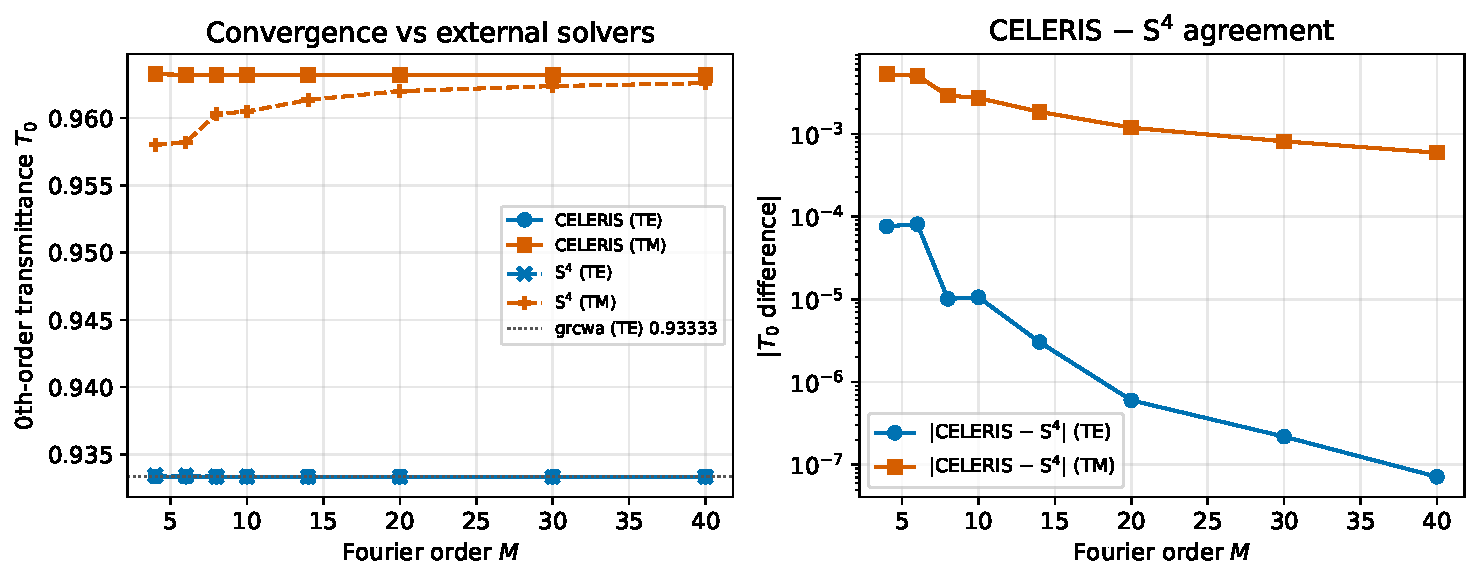
\includegraphics[width=\textwidth]{figures/fig_validation.pdf}
\caption{CELERIS vs Stanford~S$^4$ on an identical freestanding grating. Left:
0th-order transmittance vs Fourier order $M$ --- CELERIS (TE) and S$^4$ (TE) sit on
\texttt{grcwa}'s $0.93333$. Right: the CELERIS$-$S$^4$ difference falls to
$7\times10^{-8}$ (TE). In TM, CELERIS (Li's inverse rule) is within $3\times10^{-5}$
of its $M=40$ value by $M=6$, while S$^4$ with default settings approaches the same
value slowly ($6\times10^{-4}$ apart at $M=40$).}
\label{fig:validation}
\end{figure}

The end-to-end pipeline is exercised in Figs.~\ref{fig:library}--\ref{fig:psf}: sweeping
a TiO$_2$ square-pillar's fill builds the phase library (Fig.~\ref{fig:library}), and
designing a numerical-aperture (NA) ${\approx}0.2$ focusing lens from it yields a
diffraction-limited focal spot at the $\lambda f/D$ scale (Fig.~\ref{fig:psf}).

\begin{figure}[t]
\centering
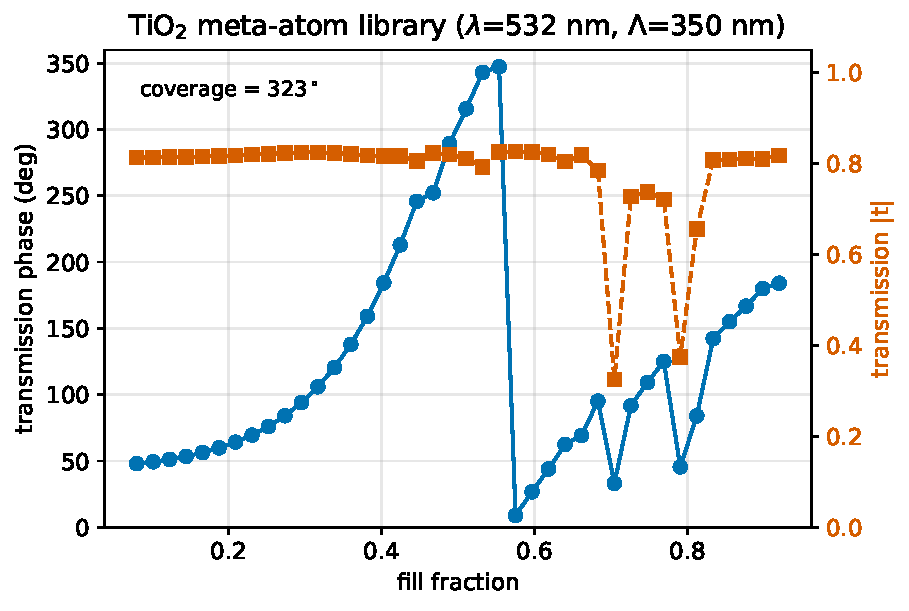
\includegraphics[width=0.8\textwidth]{figures/fig_library.pdf}
\caption{Meta-atom phase library: transmission phase and amplitude $|t|$ vs pillar fill
for a TiO$_2$ square pillar ($\lambda = 532$~nm, $\Lambda = 350$~nm, $H = 600$~nm).}
\label{fig:library}
\end{figure}

\begin{figure}[t]
\centering
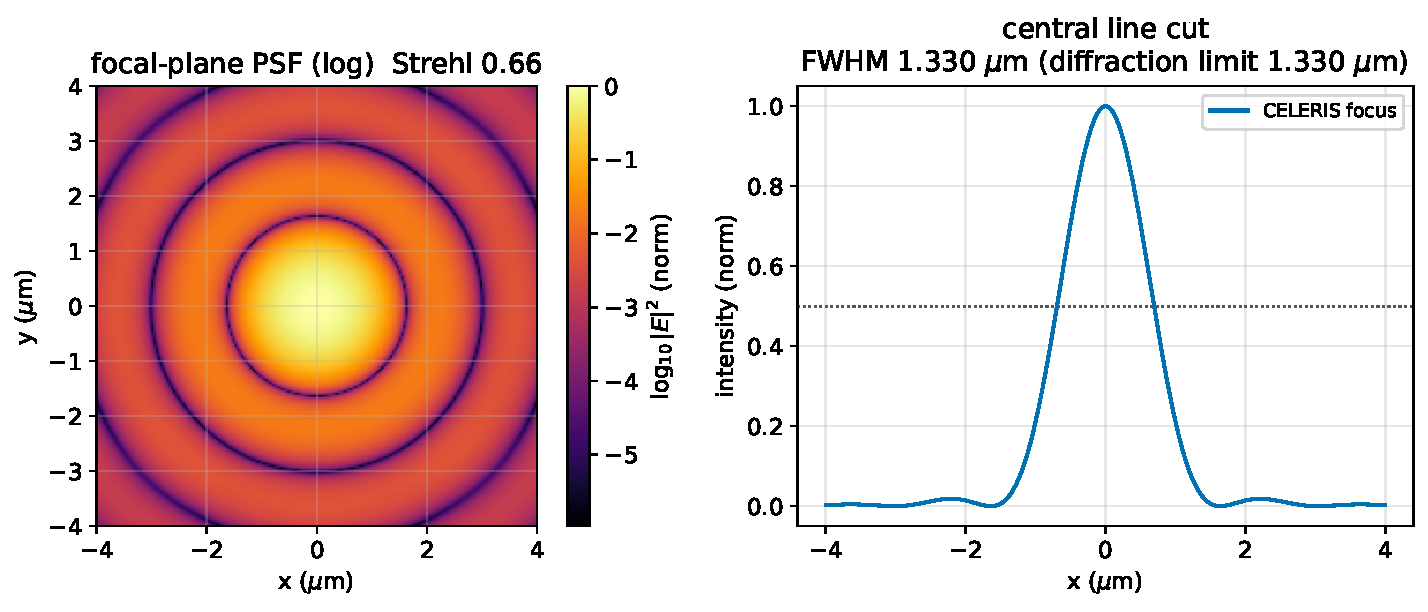
\includegraphics[width=\textwidth]{figures/fig_psf.pdf}
\caption{Focal-plane PSF of the designed lens (log scale, left) and its central line
cut (right): FWHM $= 1.330~\mu$m, consistent with the diffraction limit ($\sim\lambda f/D$).}
\label{fig:psf}
\end{figure}

The full pipeline is demonstrated by reproducing two canonical published devices end
to end:
\begin{itemize}
\item Khorasaninejad et al., \emph{Science} \textbf{352}, 1190 (2016)
      \cite{khorasaninejad2016} --- an NA${=}0.80$ Pancharatnam--Berry TiO$_2$ nanofin
      metalens. CELERIS solves the published nanofin geometry with the deposited
      atomic-layer-deposition (ALD) TiO$_2$ optical constants and recovers
      near-ideal half-wave-plate behavior
      (transmitted-normalized conversion 96--99\%), an exact geometric phase, and a
      diffraction-limited focal spot.
\item Chen et al., \emph{Nat.\ Nanotechnol.} \textbf{13}, 220 (2018) \cite{chen2018}
      --- a broadband achromatic visible metalens. CELERIS reproduces the central
      physical limit (the required group-delay span, ${\sim}4.4$~fs, exceeds the
      ${\sim}2.6$~fs a single-etch $600$~nm nanofin library spans, so the aperture is
      group-delay-limited) and, via
      single-etch group-delay engineering on a birefringent Pancharatnam--Berry library,
      cuts the chromatic focal drift of the full-scale device ($D{=}26.4~\mu$m,
      $f{=}64.7~\mu$m) from $22.7$ to $7.3~\mu$m relative to a dispersion-blind lens
      built from the same library (Fig.~\ref{fig:achromatic}).
\end{itemize}

\begin{figure}[t]
\centering
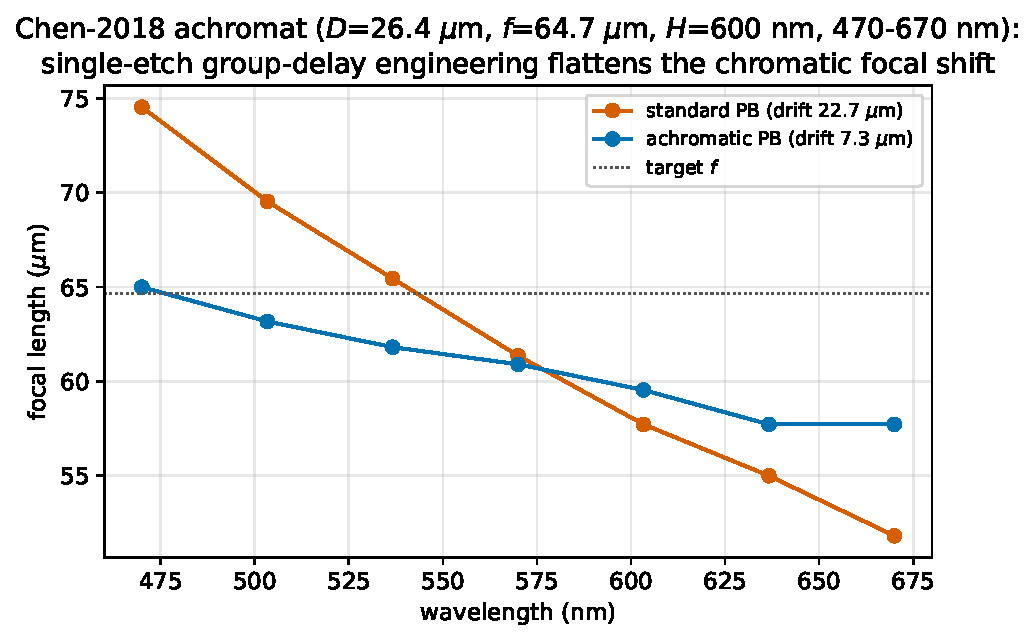
\includegraphics[width=0.8\textwidth]{figures/fig_achromatic.pdf}
\caption{Broadband achromatic metalens at the \emph{full} Chen-2018 device scale
(NA${=}0.20$, $D{=}26.4~\mu$m, $f{=}64.7~\mu$m, one $H{=}600$~nm etch, 470--670~nm):
rigorous focal length vs wavelength for a standard Pancharatnam--Berry lens and a
group-delay-engineered achromatic lens built from the \emph{same} single-etch
birefringent library. Group-delay matching cuts the chromatic focal drift from
$22.7~\mu$m to $7.3~\mu$m (results unchanged between $M{=}6$ and $M{=}8$), at the cost
of mean circular-conversion efficiency ($0.52\to0.31$), because the atoms that
supply the needed group delay convert less. The residual drift is the group-delay
design limit in action: at this aperture the required group-delay span
($\sim$$4.4$~fs) exceeds what one $600$~nm nanofin library spans ($\sim$$2.6$~fs), so
the achromat corrects only as far as the single-etch ceiling allows.
The library and the focal model keep only the zeroth diffraction order. The
$400$~nm cell is not subwavelength in the BK7 substrate below $\lambda\approx608$~nm
($\lambda < P\,n_\mathrm{sub}$): at $470$~nm the atoms send on average $25\%$ of the
incident power into substrate orders that leave at an angle and miss the focus, falling
to $6\%$ at $603$~nm and zero above $608$~nm. The drift figures are results within
the zeroth-order model; the R1 study uses $P<\lambda_\mathrm{min}/n_\mathrm{sub}$.}
\label{fig:achromatic}
\end{figure}

%% ---------------------------------------------------------------------------
\section{Performance}
\label{sec:performance}
The GPU accelerates far-field propagation only; the RCWA modal solve runs on the CPU.
We benchmark the propagation kernel (single precision) against CELERIS's own
multithreaded CPU propagation (\texttt{propagate\_pillars\_cpu}, double precision,
parallel over focal-plane rows on all 22 hardware threads of an Intel Core Ultra~9 185H)
using the built-in \texttt{psfbench} command on an RTX~4070 laptop GPU. Each timing is the
best of up to three runs, and the GPU is warmed up first so device initialization is not
timed. The double-precision CPU sum serves as the accuracy reference: the peak-normalized
single-precision PSF agrees with it to at most $4.2\times10^{-5}$, and the peak intensity
to $<2\times10^{-5}$ relative. Results are in Table~\ref{tab:perf}.

\begin{table}[t]
\centering
\caption{Far-field propagation: GPU (RTX~4070 laptop, single precision) vs the
multithreaded CPU path (Core Ultra~9 185H, 22 threads, double precision).}
\label{tab:perf}
\begin{tabular}{lcccc}
\toprule
Aperture (pillars) & Focal grid & CPU & GPU & Speedup \\
\midrule
92\,k  & $161^2$  & 3.7~s   & 31~ms  & 118$\times$ \\
92\,k  & $321^2$  & 15.1~s  & 107~ms & 141$\times$ \\
92\,k  & $641^2$  & 74.8~s  & 391~ms & 192$\times$ \\
92\,k  & $1024^2$ & 156~s   & 981~ms & 159$\times$ \\
256\,k & $161^2$  & 10.3~s  & 88~ms  & 117$\times$ \\
577\,k & $161^2$  & 25.2~s  & 189~ms & 133$\times$ \\
\bottomrule
\end{tabular}
\end{table}

On this hardware the GPU is therefore two orders of magnitude faster than a
well-parallelized CPU implementation of the same sum, roughly independent of problem
size. The CPU timings come from a laptop and vary by up to ${\sim}25\%$ between runs with
thermal and power state, so the speedups should be read as ${\sim}120$--$190\times$
rather than as precise ratios.

The dominant cost, however, is the RCWA modal solve, not propagation. The solve is
bounded by dense complex linear algebra (operator assembly, matrix inverses, and the
S-matrix recursion), which an optional Intel MKL backend accelerates. Because CELERIS
parallelizes its unit-cell sweeps across cores itself, MKL is pinned to a single thread
to avoid nested oversubscription; composed this way it is $2.3\times$ faster than the
default header-only (AVX2 SIMD) build on an $M=8$ metalens library design
(5.9~s vs 13.5~s, 16-core), with larger
gains at higher Fourier order. The default build has no MKL dependency (header-only
Eigen with AVX2); MKL is opt-in.

%% ---------------------------------------------------------------------------
\section{Application: the single-etch achromatic limit}
\label{sec:r1}
Section~\ref{sec:method} showed that the group-delay span of a library caps the
aperture of an achromat (Eq.~\eqref{eq:gdspan}), and Sec.~\ref{sec:validation} showed
the cap at work in the Chen~2018 device. This section asks how large that span is for
single-etch libraries in general, and how close it comes to the delay--bandwidth bound
of Presutti and Monticone~\cite{presutti2020}. It uses only the public CELERIS API: the
sweep and analysis scripts are in \texttt{research/r1/} of the repository, and every
number below is regenerated by them.

\subsection{Metric}
The \emph{delay span} of a library is $\Delta\tau_\mathrm{lib}=\max\tau-\min\tau$ over
the atoms kept by CELERIS's quality filters, where $\tau$ is each atom's fitted group
delay (the least-squares slope of the unwrapped phase of $t$ or $a_\times$ across the
band). Setting $\Delta T=\Delta\tau_\mathrm{lib}$ in Eq.~\eqref{eq:gdspan} and solving
for the diameter gives
\begin{equation}
D_\mathrm{lib} = 2f\sqrt{\left(1+\frac{c\,\Delta\tau_\mathrm{lib}}{f}\right)^2-1},
\label{eq:dlib}
\end{equation}
which is Eq.~15 of Buisine et al.~\cite{buisine2026}. Presutti and Monticone bound the
delay--bandwidth product of a linear, passive, time-invariant structure. For a
guided-wave structure of thickness $H$ (Tucker's form of the bound) this gives
\begin{equation}
\Delta\tau_\mathrm{PM} = \frac{H\,(n_\mathrm{max}-n_\mathrm{min})}{c}\,
\frac{\omega_c}{\Delta\omega},
\label{eq:pm}
\end{equation}
with $n_\mathrm{max}$ the pillar index and $n_\mathrm{min}=1$ the background (air) index,
both at the band centre. The first factor is the delay difference of a
non-dispersive delay line, $\Delta\tau_\mathrm{DL}$. We report
$\eta_\mathrm{DL}=\Delta\tau_\mathrm{lib}/\Delta\tau_\mathrm{DL}$, which can exceed one
through guided-mode dispersion, and
$\eta_\mathrm{PM}=\Delta\tau_\mathrm{lib}/\Delta\tau_\mathrm{PM}
=\eta_\mathrm{DL}\,\Delta\omega/\omega_c$, which must not. For the band used here,
$470$--$670$~nm with $\omega_c$ the band centre in frequency, $\Delta\omega/\omega_c=0.351$.
So a pure delay line ($\eta_\mathrm{DL}=1$) reaches $\eta_\mathrm{PM}=0.35$, and anything
above that needs frequency-dependent delay. A value $\eta_\mathrm{PM}>1$ would signal an
aliased group delay or a resonator outside Tucker's model; none occurred.

\subsection{Libraries and settings}
The sweep covers three materials (amorphous ALD TiO$_2$~\cite{siefke2016}, LPCVD
Si$_3$N$_4$, and wurtzite GaN, ordinary ray), each on its usual substrate (fused
silica for TiO$_2$ and Si$_3$N$_4$, sapphire for GaN), six etch heights
$H=0.4$--$1.5~\mu$m, and both phase mechanisms: propagation phase (``prop'': square and
circular pillars, 12 fills) and Pancharatnam--Berry (``PB'': a $12\times12$ grid of
rectangles, phase from rotation). That is 36 libraries. The period is the largest
$10$~nm step below $0.95\,\lambda_\mathrm{min}/n_\mathrm{sub}$, so no substrate order
propagates anywhere in the band: $300$~nm on silica and $250$~nm on sapphire. An
assumed $60$~nm minimum feature and gap limit the fill to $0.20$--$0.80$ at $300$~nm
and $0.24$--$0.76$ at $250$~nm. Each library is solved at 7 band points with $M=6$.
Diameters use $f=64.67~\mu$m, the NA~0.20 Chen~2018 lens. Efficiency is kept as a second
axis: the span is computed among atoms whose mean amplitude (mean $|t|$ for prop, mean
$|a_\times|$ for PB) exceeds a threshold from 0.30 to 0.90.

\paragraph{Convergence}
Every library was rebuilt with $2N-1=13$ band points. The largest span change at any
threshold was $0.88$~fs (TiO$_2$ PB, $H=0.8~\mu$m), then $0.50$ and $0.47$~fs (TiO$_2$
PB at $1.0$ and $1.5~\mu$m); every other library moved by at most $0.46$~fs. For Fourier
order, the $H=1.0~\mu$m library of each material and kind was rerun at $M=8$ and $M=10$.
The PB and the Si$_3$N$_4$ and GaN prop spans moved by at most $0.11$~fs. The TiO$_2$
prop spans moved by up to $0.34$~fs with mixed sign, so all six TiO$_2$ prop libraries
were rerun at $M=10$ and are quoted at $M=10$ ($\pm0.15$~fs).

\subsection{Delay span against the bound}
Table~\ref{tab:r1span} lists the span and $\eta_\mathrm{PM}$ at threshold 0.30, the
CELERIS default.

\begin{table}[t]
\centering
\caption{Delay span $\Delta\tau_\mathrm{lib}$ (fs) and fraction of the
Presutti--Monticone bound $\eta_\mathrm{PM}$ for 36 single-etch libraries, at mean
amplitude $\ge 0.30$. Band $470$--$670$~nm. TiO$_2$ prop at $M=10$, all others at
$M=6$.}
\label{tab:r1span}
\small
\setlength{\tabcolsep}{4pt}
\begin{tabular}{l cc cc cc}
\toprule
 & \multicolumn{2}{c}{TiO$_2$ / SiO$_2$} & \multicolumn{2}{c}{Si$_3$N$_4$ / SiO$_2$}
 & \multicolumn{2}{c}{GaN / Al$_2$O$_3$} \\
\cmidrule(lr){2-3}\cmidrule(lr){4-5}\cmidrule(lr){6-7}
$H$ ($\mu$m) & prop & PB & prop & PB & prop & PB \\
\midrule
0.4 & 3.70 / .68 & 2.33 / .43 & 1.89 / .47 & 0.51 / .13 & 2.22 / .41 & 1.12 / .21 \\
0.6 & 4.59 / .56 & 3.21 / .39 & 2.35 / .39 & 1.36 / .23 & 4.15 / .52 & 2.81 / .35 \\
0.8 & 5.93 / .54 & 5.97 / .55 & 3.37 / .42 & 2.44 / .31 & 4.47 / .42 & 3.32 / .31 \\
1.0 & 7.05 / .52 & 6.28 / .46 & 3.81 / .38 & 2.93 / .29 & 5.99 / .45 & 4.63 / .35 \\
1.2 & 8.92 / .55 & 7.83 / .48 & 4.49 / .37 & 3.48 / .29 & 6.45 / .40 & 5.32 / .33 \\
1.5 & 10.52 / .52 & 9.01 / .44 & 5.43 / .36 & 4.60 / .31 & 8.23 / .41 & 7.59 / .38 \\
\bottomrule
\end{tabular}
\end{table}

Four observations follow.
\begin{enumerate}
\item \textbf{The fraction of the bound plateaus with height.} For $H\ge0.8~\mu$m the span
      grows roughly in proportion to $H$, and $\eta_\mathrm{PM}$ stays nearly flat for each
      material and kind. Thin PB libraries fall well short ($\eta_\mathrm{PM}=0.13$--$0.43$
      at $H=0.4~\mu$m), because short pillars cannot reach half-wave retardance and few
      atoms pass the filter.
\item \textbf{The plateau is near $\eta_\mathrm{PM}\approx0.3$--$0.55$}, that is, near or
      modestly above the pure-delay-line value 0.35. No library approaches the bound.
      The highest values belong to TiO$_2$, whose prop libraries reach
      $\eta_\mathrm{DL}\approx1.5$ through guided-mode dispersion.
\item \textbf{The GaN--TiO$_2$ gap is a substrate effect, not a material one.} GaN and
      TiO$_2$ have almost the same index at the band centre (2.41 and 2.43), yet GaN's PB
      plateau is lower. A control run at $H=1.0~\mu$m swapped the substrates. PB TiO$_2$
      on sapphire fell from 0.461 to 0.370, and PB GaN on silica rose from 0.345 to 0.440.
      On the same substrate the two materials differ by at most 0.025. The prop libraries
      move the same way but less. In this sweep ``substrate'' also fixes the period and
      the fill range, and the control does not separate the three. A shorter period
      narrows the usable fill at fixed fabrication limits, which is the likely lever, but
      that was not tested.
\item \textbf{Most of the PB span costs efficiency.} At threshold 0.70 the PB spans
      collapse to at most $1.5$~fs, except Si$_3$N$_4$ at $H=1.5~\mu$m ($3.2$~fs), and
      several PB libraries keep no usable span at all. The prop spans lose at most about
      20\% up to 0.70.
      The two amplitudes are not the same quantity (conversion against transmission), so
      this compares the shape of each trade-off, not its level.
\end{enumerate}

\subsection{Achievable aperture}
$D_\mathrm{lib}$ assumes that any delay in the span can be used at any base phase. A
design needs both at once, at every radius. To test this, CELERIS's atom picker (the
one behind \texttt{design\_\allowbreak achromatic\_\allowbreak metalens} and
\texttt{design\_\allowbreak pb\_\allowbreak achromatic\_\allowbreak metalens}) was applied to each library at a series of
diameters $D=4$, 8, 12, 16, 20, 26.4, 32 and $40~\mu$m at the fixed $f$ above,
and the on-axis Strehl ratio at each band wavelength was computed from the picked atoms'
band responses $u_s(\lambda)$,
\begin{equation}
S(\lambda) = \frac{\bigl|\sum_s u_s(\lambda)\,e^{ik\,\mathrm{sag}_s}\bigr|^2}
                  {\bigl(\sum_s |u_s(\lambda)|\bigr)^2},
\end{equation}
with the free phase and group-delay offsets scanned. The achievable aperture $D_S$ is the
largest diameter whose band-minimum $S$ stays $\ge0.8$ (the Mar\'echal criterion). Each
library gets two designs: a standard, dispersion-blind pick and an achromatic pick that
also matches the group delay. $S$ is normalized by $\sum_s|u_s|$, so it measures focus
quality, not throughput. Table~\ref{tab:r1ds} gives the results at $H=1.0~\mu$m and the
range over $H=0.6$--$1.5~\mu$m.

\begin{table}[t]
\centering
\caption{Span-based diameter $D_\mathrm{lib}$ against the Strehl-based achievable
aperture $D_S$ ($\mu$m) for the standard (std) and achromatic (achr) designs, at
$H=1.0~\mu$m and as a range over $H=0.6$--$1.5~\mu$m. $D_S$ is a lower bound to the next
point of the diameter grid. TiO$_2$ prop at $M=10$. The TiO$_2$ PB range omits
$H=1.5~\mu$m (see text).}
\label{tab:r1ds}
\small
\setlength{\tabcolsep}{5pt}
\begin{tabular}{l ccc ccc}
\toprule
 & \multicolumn{3}{c}{$H=1.0~\mu$m} & \multicolumn{3}{c}{$H=0.6$--$1.5~\mu$m} \\
\cmidrule(lr){2-4}\cmidrule(lr){5-7}
library & $D_\mathrm{lib}$ & std & achr & $D_\mathrm{lib}$ & std & achr \\
\midrule
\multicolumn{7}{l}{\emph{propagation phase}} \\
TiO$_2$ / SiO$_2$       & 33 & 4  & 16 & 27--41 & 4--8   & 12--16 \\
Si$_3$N$_4$ / SiO$_2$   & 24 & 12 & 20 & 19--29 & 4--16  & 16--20 \\
GaN / Al$_2$O$_3$       & 31 & 8  & 16 & 26--36 & 4--12  & 16--20 \\
\multicolumn{7}{l}{\emph{Pancharatnam--Berry}} \\
TiO$_2$ / SiO$_2$       & 31 & 20 & 32 & 22--35 & 20     & 26.4--32 \\
Si$_3$N$_4$ / SiO$_2$   & 21 & 20 & 32 & 15--27 & 20     & 26.4--32 \\
GaN / Al$_2$O$_3$       & 27 & 20 & 32 & 21--35 & 20     & 26.4--32 \\
\bottomrule
\end{tabular}
\end{table}

\begin{itemize}
\item \textbf{The span overstates the prop achromat by about a factor of two.} Prop
      achromats reach $D_S=12$--$20~\mu$m against $D_\mathrm{lib}=19$--$41~\mu$m. A
      propagation-phase atom must supply the base phase and the group delay together, and
      most of the span is not available at the phase a given radius needs. This agrees
      with Buisine et al.~\cite{buisine2026}, who find that in the exactly achromatic
      regime the aperture is set by the atoms' ability to realize phase and dispersion
      together.
\item \textbf{PB achromats reach about $D_\mathrm{lib}$ or more} ($26.4$--$32~\mu$m for
      $H\ge0.6~\mu$m; where $D_\mathrm{lib}$ is larger, the grid does not resolve the
      difference). The rotation sets the base phase, so the whole span is usable, and
      $S\ge0.8$ tolerates some group-delay mismatch.
\item \textbf{A dispersion-blind PB lens reaches $20~\mu$m in every library}, more than
      most prop achromats. This is also a check: the standard PB pick uses the same atom
      everywhere, so its Strehl curve depends only on the geometric phase and must be the
      same for every library. It is ($S_\mathrm{min}=0.817$ at $20~\mu$m, $0.532$ at
      $26.4~\mu$m).
\item \textbf{Standard prop designs get worse with height}, down to $4~\mu$m for
      $H\ge1.2~\mu$m in every material, because taller
      atoms are more dispersive and a dispersion-blind pick turns that into focal error.
\end{itemize}
The scan's Python copy of the picker reproduces the C++ designs atom for atom at
$D=10$ and $25~\mu$m for every library. Rerunning the TiO$_2$ prop libraries at $M=10$
changes $D_S$ by one grid step in two cases. The substrate controls give the same $D_S$
for PB and differ by one grid step for prop. One case is excluded: the TiO$_2$ PB library at
$H=1.5~\mu$m gives an achromatic $D_S$ of only $20~\mu$m, but its atoms' group delays move
by up to $3.3$~fs under band refinement, so 7 band samples do not resolve its strongly
resonant atoms and the value is not reliable.

\paragraph{Scope of the result}
The lens model is locally periodic: each site uses the response of its atom in an
infinite array, and the focus is computed from those responses. It is not a full-wave
simulation of the finite lens. The diameter grid is coarse, so $32$ and $40~\mu$m are not
resolved. The fabrication limits ($60$~nm feature and gap) are round numbers, not those
of a specific process. Within these limits the study shows what the integrated pipeline
is for: the span, the bound, the designed lens and its Strehl ratio come from one
library and one data model, and the comparison between them (here, that span-based
estimates overstate propagation-phase achromats) is only visible when all four are
computed together.

%% ---------------------------------------------------------------------------
\section{Limitations}
\begin{itemize}
\item \textbf{The RCWA eigensolve is CPU-only.} The GPU accelerates far-field
      propagation, not the modal solve. A GPU eigensolve was prototyped (cuSOLVER) and
      found no faster than the CPU path; the promising direction is batching the many
      independent unit-cell solves of a library, which is future work.
\item \textbf{Inverse design uses finite-difference optimization} over low-dimensional
      parametric meta-atoms; an analytic adjoint (true gradient-based / differentiable
      RCWA) is planned.
\item \textbf{Curved shapes (circle/ellipse) converge slowly} (staircasing of a curved
      interface), a known RCWA property confirmed against \texttt{grcwa}.
\item \textbf{Achromatic multi-height designs imply a grayscale/multi-level etch}; the
      single-etch Pancharatnam--Berry variant is the directly fabricable one.
\item \textbf{Lens-level analysis is locally periodic.} Each site uses the response of
      its atom in an infinite array; coupling between dissimilar neighbours and the
      finite aperture are not simulated full-wave.
\item \textbf{Scope is metalenses/metasurfaces via RCWA} --- explicitly not FDTD or ray
      tracing.
\end{itemize}

%% ---------------------------------------------------------------------------
\section{Conclusions}
CELERIS is a from-scratch, validated implementation of the complete metalens design
workflow --- rigorous RCWA/FMM solver, meta-atom library builder, phase-mapping and
inverse-design layer, optical analysis battery, GPU-accelerated far-field
propagation, and GDSII export --- delivered as one native package scriptable from
C++, a CLI, and Python. Its correctness is enforced by a locked self-test suite
whose tolerances are checked against closed-form physics, energy conservation, and
the independent solvers \texttt{grcwa} and Stanford~S$^4$ (agreement to
$\sim$$7\times10^{-8}$ on an identical grating), and its utility is demonstrated by
reproducing a published TiO$_2$ metalens end to end.

The methodological payoff of integrating these stages, rather than the integration
itself, is the paper's central point: because the library, design, and analysis
share one data model, CELERIS computes device-level quantities that a solver called
in a loop cannot express --- sharply, the group-delay design limit that bounds
single-etch broadband achromats, which it recovers for a published device and maps
across 36 single-etch libraries (Sec.~\ref{sec:r1}). CELERIS
does not aim to be the fastest raw kernel; the GPU/autodiff-native solvers remain
stronger at the bare solve. The natural next steps close that gap along the axes
identified in Limitations: an analytic adjoint for differentiable, gradient-based
inverse design, and a GPU-batched library solve. The tool is released under Apache-2.0
and archived on Zenodo so that both the pipeline and every reported number are
reproducible.

%% ---------------------------------------------------------------------------
\section*{CRediT authorship contribution statement}
\textbf{Amarnath Patel:} Conceptualization, Methodology, Software, Validation,
Investigation, Data curation, Writing -- original draft, Writing -- review \& editing.

\section*{Declaration of competing interest}
The author declares no known competing financial interests or personal relationships
that could have appeared to influence the work reported in this paper.

\section*{Funding}
This research received no specific grant from funding agencies in the public,
commercial, or not-for-profit sectors.

\section*{Data availability}
CELERIS is open source under the Apache License 2.0. The source code, the locked
self-test suite, and the scripts that regenerate every figure and table in this paper
are available on GitHub (\url{https://github.com/jeebuscrossaint/CELERIS}). Release
v1.0.0 is archived at Zenodo (\url{https://doi.org/10.5281/zenodo.21891346}); it predates
the study of Sec.~\ref{sec:r1}. The numbers of that section were computed between
commits \texttt{baa9af0} (2026-11-19) and \texttt{474fd82} (2026-11-25). Across that
range the solver is unchanged: the commits add only the scripts in \texttt{research/r1/}
and one Python accessor for the PB band response. Running those scripts at commit
\texttt{474fd82} regenerates them.

%% ---------------------------------------------------------------------------
\section*{Declaration of generative AI in the writing process}
During the preparation of this work the author used Anthropic Claude to assist with
software implementation, the scripts of the study in Sec.~\ref{sec:r1}, and manuscript
drafting. The author reviewed and edited all output, made every design and physics
decision, and takes full responsibility for the content. All numerical results in
Secs.~\ref{sec:validation}--\ref{sec:performance} are enforced by the validation suite
described above, and those in Sec.~\ref{sec:r1} are regenerated by the scripts in
\texttt{research/r1/}.

%% ---------------------------------------------------------------------------
\bibliographystyle{elsarticle-num}
\bibliography{../paper}

\end{document}
